

\chapter{\label{appendix:fet_gnr_hybrid}Porphyrin--GNR Hybrid Field-Effect Transistors}

\minitoc

\section{Additional Data}\label{sec:appendix:gnr_hybrid}
Here below we report additional data for the \glspl{pGNR}



\newpage

\begin{figure}[hbtp]
    \begin{center}
        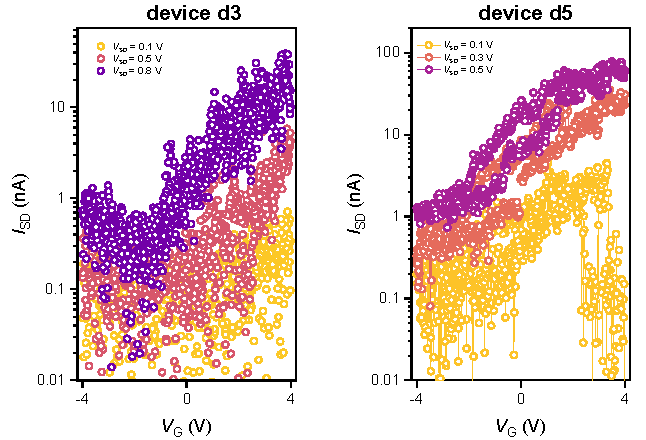
\includegraphics[width=\textwidth]{text/d3_d5.pdf}
        \caption[MGNR--Ni Hybrid: Additional FETs (device d3, d5)]
        {
            \textbf{left,} \gls{FET} characteristics:  $I_\textrm{on}/I_\textrm{off}\simeq 10^1$ at $V_\textrm{SD}=\SI{0.1}{\volt}$, $SS\simeq\SI{3}{\volt}$~dec$^{-1}$ at $V_\textrm{SD}=\SI{0.6}{\volt}$, slightly n-doped, poor off ($I_\textrm{off}\simeq\SI{0.1}{\nano\ampere}$) and on ($I_\textrm{on}\simeq\SI{5}{\nano\ampere}$) currents.
            \textbf{right,} \gls{FET} characteristics:  $I_\textrm{on}/I_\textrm{off}\simeq 10^2$ at $V_\textrm{SD}=\SI{0.5}{\volt}$, $SS\simeq\SI{1.5}{\volt}$~dec$^{-1}$ at $V_\textrm{SD}=\SI{0.3}{\volt}$, n-doped, poor off ($I_\textrm{off}<\SI{1}{\nano\ampere}$) and on ($I_\textrm{on}\simeq\SI{15}{\nano\ampere}$) currents.
        }
    \end{center}
\end{figure}

\newpage

\begin{figure}[hbtp]
    \begin{center}
        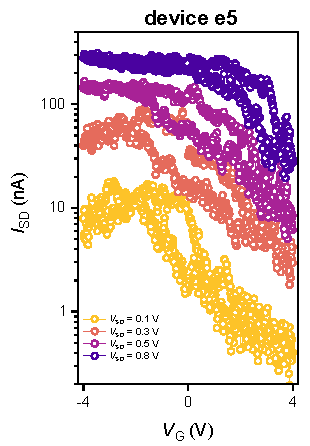
\includegraphics[width=0.5\textwidth]{text/e5.pdf}
        \caption[MGNR--Ni Hybrid: Additional FETs (device e5)]
        {
            \gls{FET} characteristics:  $I_\textrm{on}/I_\textrm{off}\simeq 10^2$ at $V_\textrm{SD}=\SI{0.1}{\volt}$ ($I_\textrm{on}/I_\textrm{off}\simeq 10^1$ at $V_\textrm{SD}=\SI{0.8}{\volt}$), small hysteresis present in all the transfer characteristics, $SS\simeq\SI{400}{\milli\volt}$~dec$^{-1}$ at $V_\textrm{SD}=\SI{0.8}{\volt}$, $\mu_\textrm{lin}=\SI{5}{\centi\metre\squared\per\volt\per\second}$,  $\mu_\textrm{sat}=\SI{1}{\centi\metre\squared\per\volt\per\second}$
        }
    \end{center}
\end{figure}









